\title{Novas publicações em pedometria}
\maketitle
\begin{wrapfigure}{l}{0.15\textwidth}
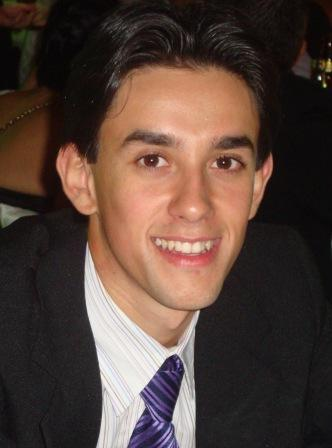
\includegraphics[width=0.15\textwidth]{figuras/foto-jean}
\end{wrapfigure}
O segundo número da nossa \textit{Newsletter} inaugura a seção de divulgação de novas publicações em pedometria. Todos podem contribuir enviando informações básicas sobre novas publicações, sejam elas nacionais ou internacionais. Basta enviar a contribuição ao editor responsável pela seção de novas puvlicações em pedometria, Jean Michel Moura-Bueno, pelo endereço de e-mail \email{bueno.jean1@gmail.com}.\\
As contribuições deverão ser sucintas, com tamanho inferior ao de um resumo geralmente apresentado em artigos científicos. Como estas contribuições servirão como propagandas de novos trabalhos publicados, é recomendado apresentar apenas informações chave, destaques que realmente chamam a atenção do leitor. Uma bom exemplo para ser seguido são os \emph{highlights} usados nos artigos da Elsevier: \emph{Os ``highlights'' são um pequeno conjunto de pontos que transmitem os resultados principais e fornecem aos leitores uma visão textual rápida do artigo}. Os resumos originais não serão publicados na \textit{Newsletter} por tal prática envolver questões de direitos dos autores e editoras das publicações originais.\\
Também é importante apresentar a forma de citação recomendada pelos autores, bem como o endereço da publicação na internet. Caso a publicação possua alguma figura interessante e autoexplicativa, a mesma deve ser enviada juntamente com o texto descritivo para a \textit{Newsletter}.
\section{Exemplo}
Abaixo há um exemplo utilizando uma publicação recente. Primeiro, é mostrado o resumo do artigo publicado no periódico científico e, em seguida, o formato recomendado para publicação na seção de novas publicações em pedometria da nossa \textit{Newsletter}.
\subsection{Título da publicação}
Building predictive models of soil particle-size distribution
\subsection{Citação}
A. Samuel-Rosa, R.S.D. Dalmolin, P. Miguel (2013) Building predictive models of soil particle-size distribution. {\em Revista Brasileira de Ciência do Solo} 37:422-430.
\subsection{Resumo original - não será publicado}
É possível construir modelos preditivos (MPs) da distribuição do tamanho de partículas do solo (DTP) em uma região que possua geologia complexa e uma superfície geomórfica jovem e instável? O principal objetivo deste trabalho foi responder a essa questão. Um conjunto de 339 amostras de solo de uma pequena bacia hidrográfica de encosta do sul do Brasil foi usado para construir MPs da DTP na camada superficial do solo. Modelos de regressão linear múltiplos foram construídos com atributos de terreno (elevação, declividade, área de captação, índice de convergência, índice de umidade topográfica). Os MPs explicaram mais da metade da variância dos dados. Esse desempenho é semelhante (se não melhor) ao da abordagem tradicional de mapeamento de solos. Para algumas frações de tamanho, o desempenho dos MPs pode chegar a 70\%. As maiores incertezas ocorrem nas áreas de maior complexidade geológica. Assim, melhorias significativas nas predições somente poderão ser alcançadas se dados geológicos acurados forem 
disponibilizados. Enquanto isso, MPs construídos a partir de atributos de terreno são eficientes em estimar a DTP de solos de regiões com geologia complexa.
\subsection{Resumo para a \textit{Newsletter}}
É possível construir modelos preditivos da distribuição do tamanho de partículas numa região com geologia complexa (arenitos e basaltos com arenito \emph{intertrap}) e superfície geomórfica jovem e instável? Esta é a pergunta que nos fez desenvolver este estudo em uma pequena bacia hidrográfica no RS. Com um conjunto de $n=339$ observações e alguns atributos de terreno, construímos modelos lineares para predizer a distribuição do tamanho de partículas na camada superficial do solo, tratados como dados composicionais. Os resultados sugerem que o desempenho dos modelos pode ser inferior, similar ou superior ao método tradicional de mapeamento do solo. As maiores incertezas estão conectadas às áreas onde as informações geológicas são mais pobres. Destacamos que a qualidade dos mapas geológicos deve ser melhorada se predições superiores forem demandadas.
\begin{footnotesize}
\begin{thebibliography}{99}
\bibitem[Samuel-Rosa et~al. (2013) Samuel-Rosa, Dalmolin, Miguel]{Samuel-RosaEtAl:2013} 
A. Samuel-Rosa, R.S.D. Dalmolin, P. Miguel (2013)
\newblock Building predictive models of soil particle-size distribution.
\newblock {\em Revista Brasileira de Ciência do Solo} 37:422-430. [\url{http://dx.doi.org/10.1590/S0100-06832013000200013}]
\end{thebibliography}
\end{footnotesize}
\address{Jean Michel Moura-Bueno\\
  Universidade Federal de Santa Maria\\
  \email{bueno.jean1@gmail.com}}
%%% Local Variables: 
%%% mode: latex
%%% TeX-master: documento-principal.tex
%%% End: 